%                                                                 aa.dem
% AA vers. 8.2, LaTeX class for Astronomy & Astrophysics
% demonstration file
%                                                       (c) EDP Sciences
%-----------------------------------------------------------------------
%
%\documentclass[referee]{aa} % for a referee version
%\documentclass[onecolumn]{aa} % for a paper on 1 column  
%\documentclass[longauth]{aa} % for the long lists of affiliations 
%\documentclass[rnote]{aa} % for the research notes
%\documentclass[letter]{aa} % for the letters 
%\documentclass[bibyear]{aa} % if the references are not structured 
% according to the author-year natbib style

%
\documentclass[]{aa}

%
\usepackage{graphicx}
\usepackage{xcolor}
\usepackage{natbib}
\bibpunct{(}{)}{;}{a}{}{,} % to follow the A&A style
%%%%%%%%%%%%%%%%%%%%%%%%%%%%%%%%%%%%%%%%
\usepackage{txfonts}
%%%%%%%%%%%%%%%%%%%%%%%%%%%%%%%%%%%%%%%%
\usepackage{hyperref}
% To add links in your PDF file, use the package "hyperref"
% with options according to your LaTeX or PDFLaTeX drivers.
%
\begin{document} 


   \title{The GALAH Survey: Variable star - Cepheids \& RR Lyrae}

   \author{The GALAH collaboration, including S. Buder\inst{1}}

   \authorrunning{The GALAH collaboration}

   \institute{Max Planck Institute for Astronomy (MPIA), Koenigstuhl 17, D-69117 Heidelberg}

   \date{Received XX XX, 2019; accepted XX XX, 2019}
 
  \abstract{
  By selecting stars of the GALAH+\textit{Gaia} overlap with high photometric variability, we have identified 2238 stars with photometric variability in \textit{Gaia}'s G band. Selections within color-magnitude diagrams allowed us to identify 91 Cepheid and 384 RR Lyrae candidates. Looking at the coordinates of these stars, $47\%$ of the found Cepheid candidates are located in the loci of the SMC and LMC. Their distances from \cite{BailerJones2018} are ranging from 4 to $17\,\mathrm{kpc}$ but have very uncertain parallaxes, which could cause an underestimated distance due to the chosen prior. These Cepheid candidates might hence actually be located in the SMC/LMC. The $BP-RP$ color of the RR Lyrae candidates suggests that their vast majority are RR Lyrae (ab). The non-classified variable stars could include long-periodic variables (e.g. the most luminous variables) and eclipsing binaries. Combining the GALAH survey can help to identify unresolved binaries or confirm their nature via spectroscopy.}

   \keywords{}

   \maketitle
%
%________________________________________________________________

%________________________________________________________________
\section{Introduction}

One can select variable stars from the \textit{Gaia}'s photometric variability, i.e.
\begin{align} \label{eq:variability}
var = \sqrt{\textsc{n\_obs\_g\_mag}} \cdot \textsc{phot\_g\_mean\_flux\_over\_error} \\ \sim 0.25 \text{peak to peak variability}
\end{align}

%________________________________________________________________
\section{Data selection} \label{sec:selection}

\begin{enumerate}
	\item Use x-match of GALAH with \textit{Gaia} DR2, WISE, 2MASS, hereafter called "All GALAH stars".
	\item Select stars with $4\cdot variability > 0.32$ (using \autoref{eq:variability}), hereafter called "Variable stars". These are stars with high photometric variability, which in the magnitude range of GALAH stars (see Fig.~\ref{fig:figure1}) is likely to be intrinsic.
\end{enumerate}

\begin{figure}[h!]
\centering
  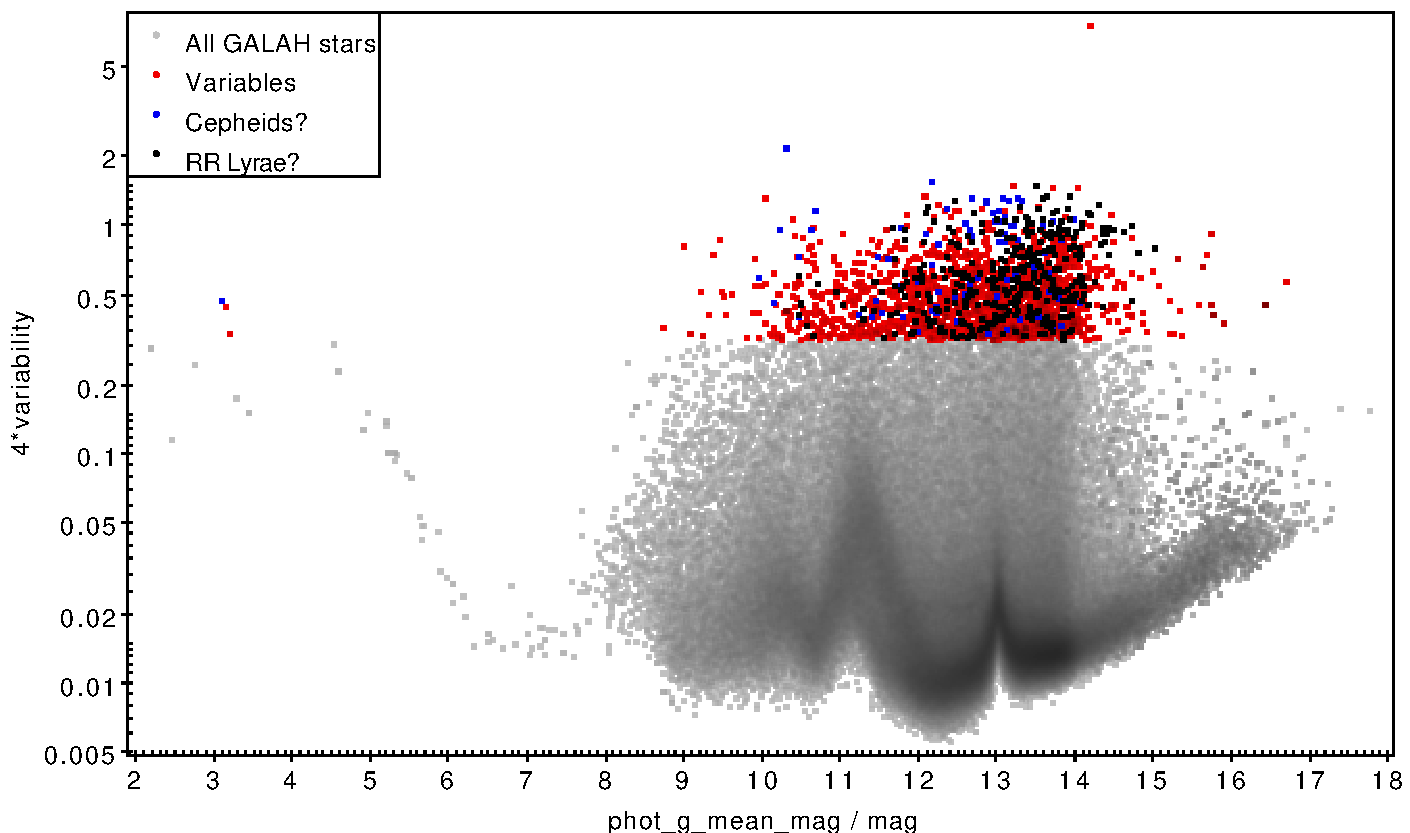
\includegraphics[width=0.45\textwidth]{Figures/variability_gmag.pdf}
    \caption{Photometric variability from \autoref{eq:variability} as a function of \textit{Gaia} G.}
    \label{fig:figure1}
\end{figure}

\paragraph{Cepheid selection}
Select a subset of the latter, hereafter called "Cepheids?", with a cut in $M_{K_S}$ and poorly dereddened 2MASS color
\begin{align} \label{eq:cepheids}
	\textsc{ks\_m} - 5 \cdot \log_{10}(\frac{\textsc{r\_est}}{10}) < -3, \\
	\textsc{j\_m} - \textsc{ks\_m} - \frac{1}{4} \cdot (\textsc{phot\_rp\_mean\_mag} - \textsc{ks\_m}) < 0.35
\end{align}

\paragraph{RR Lyrae selection}

\cite{Eyer2018} have shown that RR Lyrae can be identified at a distinct position in the \textit{Gaia} CMD.

Select another subset of the latter, hereafter called "RR Lyrae?", within a bin $M_{K_S}$ and cut in $BP-RP$
\begin{align} \label{eq:cepheids}
	\textsc{bp\_rp} < 1, \\
	-0.25 < \textsc{phot\_rp\_mean\_mag} - 5\cdot \log_{10} (\frac{\textsc{r\_est}}{10}) < 1.75
	\end{align}

The distribution of these subsets are plotted in a $T_\text{eff}$-$\log g$ diagram (Fig.~\ref{fig:figure2}), color-magnitude diagrams (Fig.~\ref{fig:figure3}) and in a sky plot (Fig.~\ref{fig:figure4}). 

\begin{figure}[h!]
\centering
  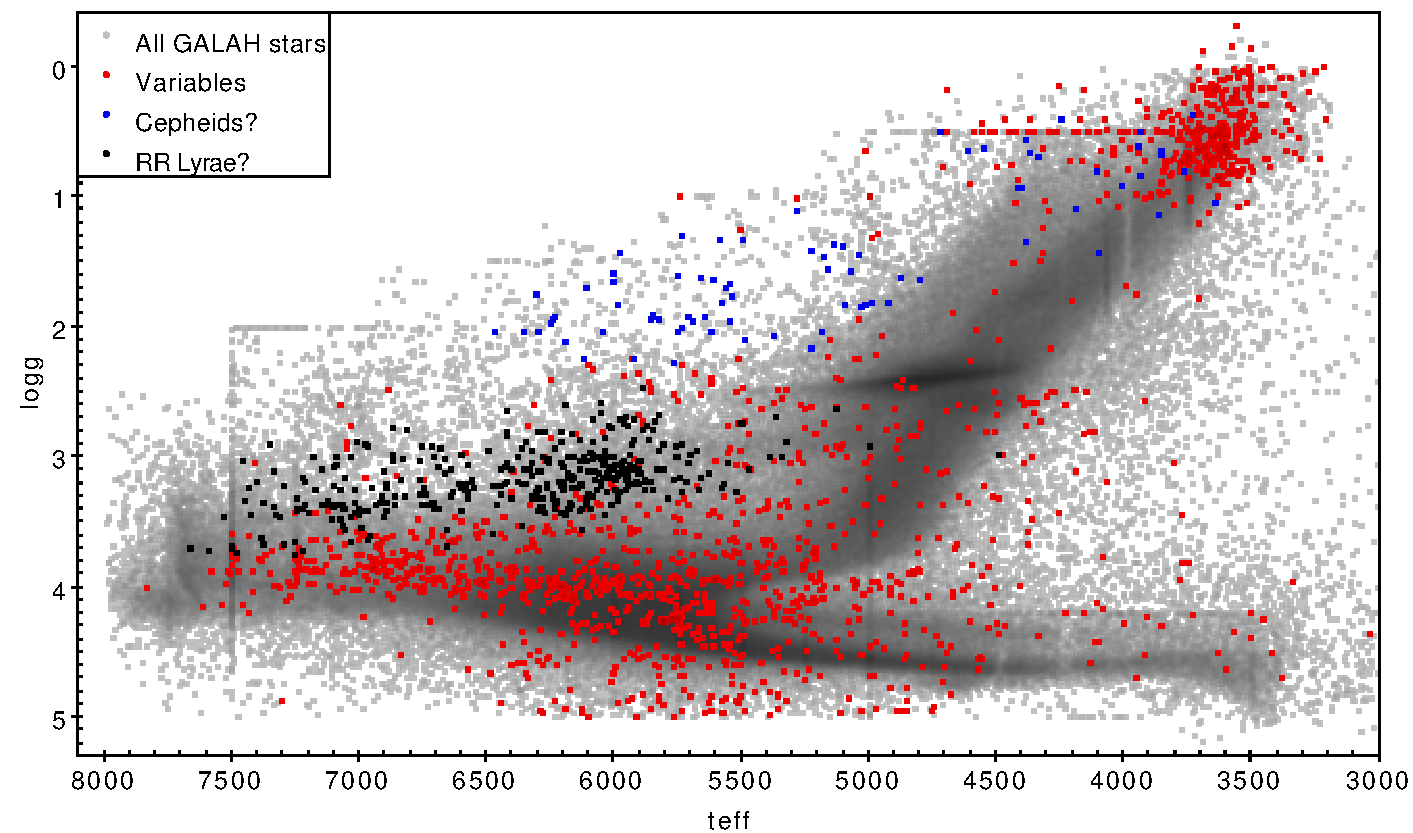
\includegraphics[width=0.45\textwidth]{Figures/variability_teff_logg.pdf}
    \caption{Spectroscopic $\log g$ as a function of $T_\text{eff}$ from GALAH iDR3.}
    \label{fig:figure2}
\end{figure}

\begin{figure*}[h!]
\centering
  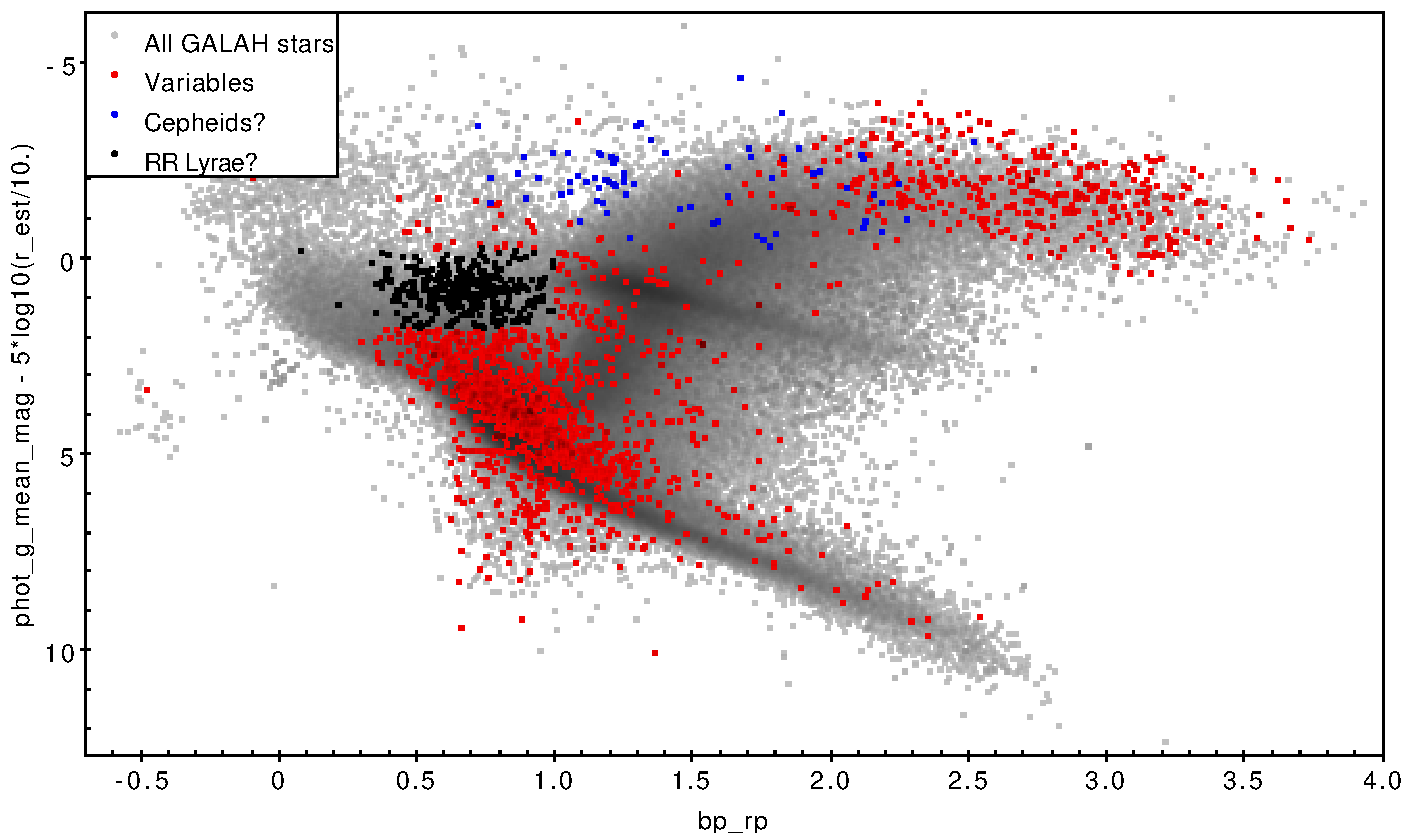
\includegraphics[width=0.6\textwidth]{Figures/variability_cmd.pdf}
  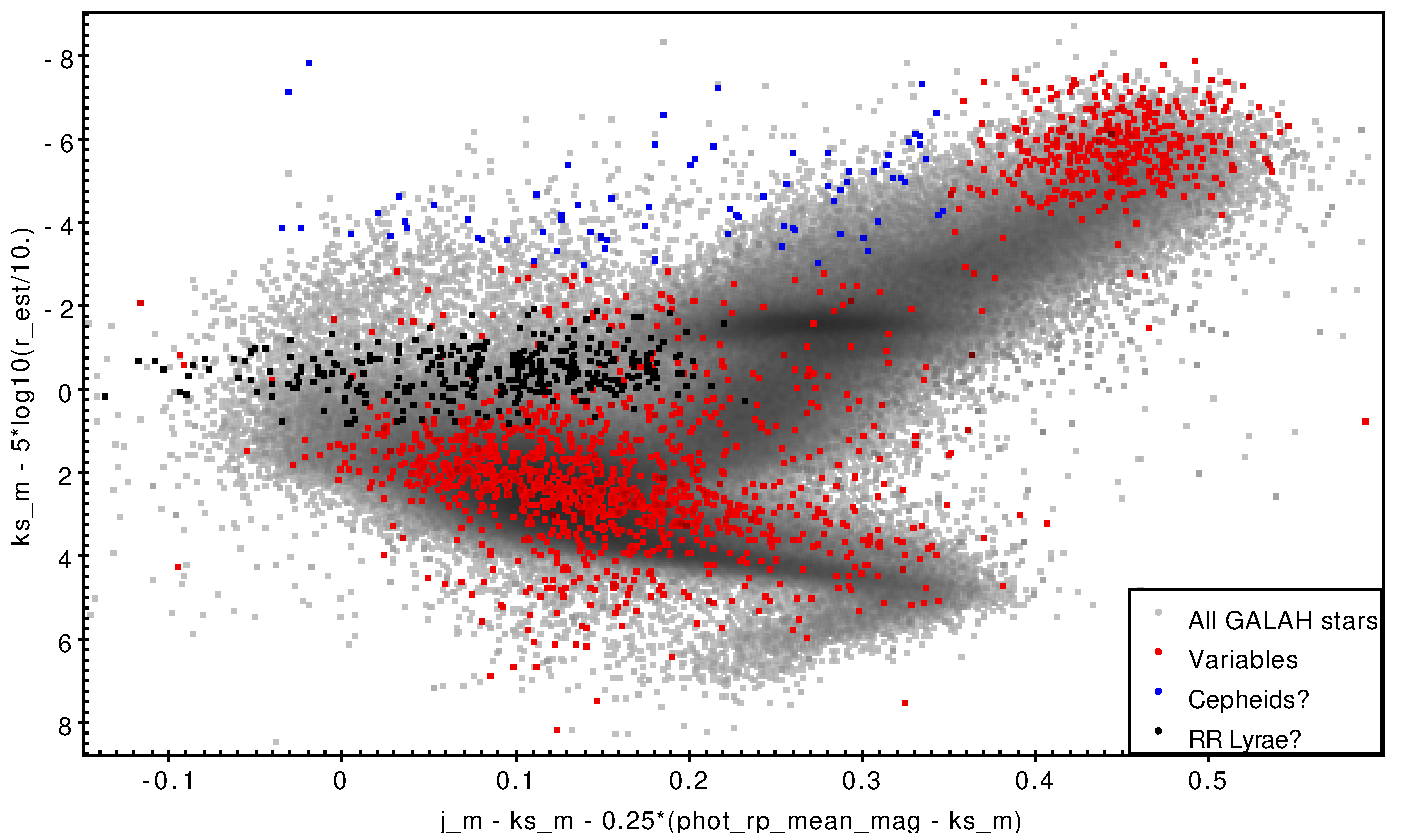
\includegraphics[width=0.6\textwidth]{Figures/variability_cmd2.pdf}  
    \caption{Color-magnitude-diagrams: $M_G$ as a function of $BP-RP$ (upper panel) and $M_{K_S}$ as a function of poorly dereddened $J - K_S$ color (lower panel).}
    \label{fig:figure3}
\end{figure*}

\begin{figure*}[h!]
\centering
  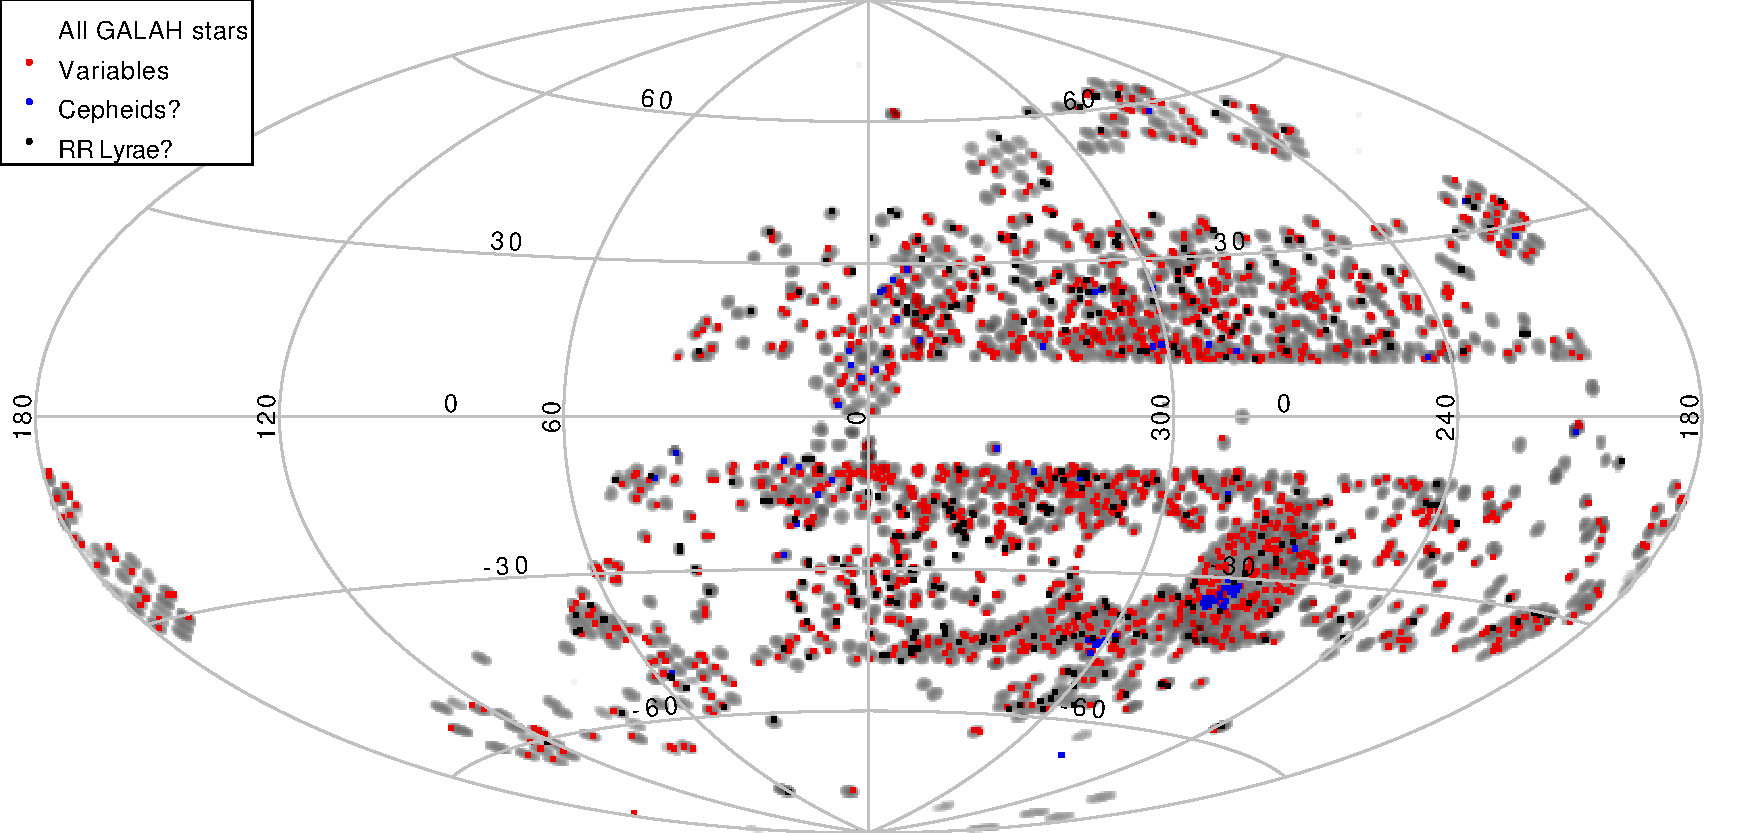
\includegraphics[width=0.9\textwidth]{Figures/variability_l_b.pdf}
    \caption{Sky distribution $(l,b)$ of "Variables", "Cepheids?", and "RR Lyraes?".}
    \label{fig:figure4}
\end{figure*}

%
%________________________________________________________________
%\section{Discussion}

%
%________________________________________________________________
%\section{Conclusions}


%-------------------------------------------------------------------

% for the bibliography, at the end
\bibstyle{aa} % style aa.bst
\bibliographystyle{aa} % style aa.bst
\bibliography{bib.bib} % your references Yourfile.bib

\label{LastPage}
\end{document}